%% This is file `elsarticle-template-1-num.tex',
%%
%% Copyright 2009 Elsevier Ltd
%%
%% This file is part of the 'Elsarticle Bundle'.
%% ---------------------------------------------
%%
%% It may be distributed under the conditions of the LaTeX Project Public
%% License, either version 1.2 of this license or (at your option) any
%% later version.  The latest version of this license is in
%%    http://www.latex-project.org/lppl.txt
%% and version 1.2 or later is part of all distributions of LaTeX
%% version 1999/12/01 or later.
%%
%% Template article for Elsevier's document class `elsarticle'
%% with numbered style bibliographic references
%%
%% $Id: elsarticle-template-1-num.tex 149 2009-10-08 05:01:15Z rishi $
%% $URL: http://lenova.river-valley.com/svn/elsbst/trunk/elsarticle-template-1-num.tex $
%%
\documentclass[preprint,12pt]{elsarticle}

%% Use the option review to obtain double line spacing
%% \documentclass[preprint,review,12pt]{elsarticle}

%% Use the options 1p,twocolumn; 3p; 3p,twocolumn; 5p; or 5p,twocolumn
%% for a journal layout:
%% \documentclass[final,1p,times]{elsarticle}
%% \documentclass[final,1p,times,twocolumn]{elsarticle}
%% \documentclass[final,3p,times]{elsarticle}
%% \documentclass[final,3p,times,twocolumn]{elsarticle}
%% \documentclass[final,5p,times]{elsarticle}
%% \documentclass[final,5p,times,twocolumn]{elsarticle}

%% The graphicx package provides the includegraphics command.
\usepackage{graphicx}
%% The amssymb package provides various useful mathematical symbols
\usepackage{amssymb}
%% The amsthm package provides extended theorem environments, I added the fleqn to have items left align
\usepackage[fleqn]{amsmath}
%%%%%%%%%Packages I have loaded
\usepackage{dcolumn}
\usepackage{natbib}
\setcitestyle{authoryear}
\setcitestyle{round}
\usepackage [english]{babel}
\usepackage [autostyle, english = american]{csquotes}
\MakeOuterQuote{"}
\usepackage{bm}
\usepackage{float}
\usepackage{lscape}
\usepackage{subcaption}
\usepackage{fancyhdr}
\usepackage{lipsum}
\usepackage{array}
\usepackage{tabu}
\usepackage[utf8]{inputenc}
\usepackage{longtable}
\usepackage{rotating} % To display tables in landscape
\usepackage{afterpage}

%% natbib.sty is loaded by default. However, natbib options can be
%% provided with \biboptions{...} command. Following options are
%% valid:

%%   round  -  round parentheses are used (default)
%%   square -  square brackets are used   [option]
%%   curly  -  curly braces are used      {option}
%%   angle  -  angle brackets are used    <option>
%%   semicolon  -  multiple citations separated by semi-colon
%%   colon  - same as semicolon, an earlier confusion
%%   comma  -  separated by comma
%%   numbers-  selects numerical citations
%%   super  -  numerical citations as superscripts
%%   sort   -  sorts multiple citations according to order in ref. list
%%   sort&compress   -  like sort, but also compresses numerical citations
%%   compress - compresses without sorting
%%
%% \biboptions{comma,round}

% \biboptions{}

\journal{GitHub}
\pagestyle{fancy}
\fancyfoot{}
\fancyfoot[C]{\thepage}
\begin{document}
\begin{frontmatter}

%% Title, authors and addresses

\title{The Impact of the Dodd-Frank Act on Community Bank Security Portfolio Selection} 

%% use the tnoteref command within \title for footnotes;
%% use the tnotetext command for the associated footnote;
%% use the fnref command within \author or \address for footnotes;
%% use the fntext command for the associated footnote;
%% use the corref command within \author for corresponding author footnotes;
%% use the cortext command for the associated footnote;
%% use the ead command for the email address,
%% and the form \ead[url] for the home page:
%%
%% \title{Title\tnoteref{label1}}
%% \tnotetext[label1]{}
%% \author{Name\corref{cor1}\fnref{label2}}
%% \ead{email address}
%% \ead[url]{home page}
%% \fntext[label2]{}
%% \cortext[cor1]{}
%% \address{Address\fnref{label3}}
%% \fntext[label3]{}


%% use optional labels to link authors explicitly to addresses:
%% \author[label1,label2]{<author name>}
%% \address[label1]{<address>}
%% \address[label2]{<address>}

\author{Alexander Wirth}

\address{Finance PhD Student, Ross School of Business \\ 
710 East University Executive Residence \\ 
Ann Arbor, MI 48109 \\ 
amwirth@umich.edu\footnote{I thank Amiyatosh Purnanandam, Uday Rajan, and Matteo Crosignani for guidance and suggestions.}}

\begin{abstract}
%% Text of abstract
Dodd-Frank restrictions on the use of credit ratings in federal regulatory documents have resulted in additional regulator scrutiny on bank security holdings.  With small banks' asset portfolios being more concentrated in local relationship-based loans than larger depository institutions, departures from security portfolio optimality make small banks and firms reliant on community bank credit more susceptible to local economic shocks.  However, a difference in difference framework using bank "Call Report" data shows small banks have not disproportionately divested from newly regulated securities.  Through the channel of bank security selection, neither large nor small bank borrowers have been more burdened by the regulation.  
\end{abstract}

\begin{keyword}
Dodd-Frank Act; Regulation; Community Banks; Relationship Lending; Small Firms
%%Science \sep Publication \sep Complicated
%% keywords here, in the form: keyword \sep keyword

%% MSC codes here, in the form: \MSC code \sep code
%% or \MSC[2008] code \sep code (2000 is the default)

\end{keyword}

\end{frontmatter}

%%
%% Start line numbering here if you want
%%
%\linenumbers


%% main text
\section{Introduction and Background}
\subsection{Background}
Community banks' loan portfolios have a larger share of small business loans than larger depository institutions, and previous literature has focused on the Dodd-Frank's impact on small businesses through the economic channel of additional regulatory costs on community banks \citep{Dahl2016,LuxRobertGreene2015,Bordo2018,Reichow2017}.  I contribute to the Dodd-Frank small business and banking literature an examination of the law's impact on bank security portfolio selection and the implications for small firms. Specifically, I question if the Office of the Comptroller of the Currency's Dodd-Frank motivated regulation requiring banks' corporate bonds, foreign debt instruments, and private structured securities to meet revised "investment grade standards" disproportionately altered small banks' securities holdings.   By analyzing U.S. banks' securities holdings in a difference in difference framework, I conclude smaller community banks have not been more burdened than larger depository institutions.

Prior to the signing of the Dodd-Frank Wall Street Reform and Consumer Protection Act, federal regulators required banks' fixed income securities investments to meet "investment grade" standards as designated by credit rating agencies.  This was a mechanism to reduce bank risk-taking to combat the well documented negative externalities of bank failure exacerbated by the the moral hazard issues of deposit insurance.  Still, the issuer pay model among credit rating agencies means a constant CRA balancing act between long-run reputation concerns \citep{Klein1981} and short-term security issuer interests \citep{Becker2011,Goel2015}.  Furthermore, only credit ratings from the Securities and Exchange Commission Nationally Recognized Statistical Ratings Organizations could be used in bank regulatory compliance.  Prior rules created a guaranteed demand among banks for NRSRO ratings, further complicating credit rating agency incentives \citep{White2018}.  With the spike in credit ratings downgrades in structured mortgage securities during the financial crisis, motivations were high to reduce reliance on NRSRO's \citep{Soroushian2016}.  In response, section 939A of the Dodd Frank Act instructed each Federal Agency "to remove any reference to or requirement of reliance on credit ratings and to substitute in such regulations such standard of credit-worthiness as each respective agency shall determine as appropriate for such regulations \citep{111thCongress2010}." 

In June of 2012, The OCC complied with section 939A by redefining "investment grade" as "the issuer of a security has an adequate capacity to meet financial commitments under the security for the projected life of the asset or exposure. An issuer has an adequate capacity to meet financial commitments if the risk of default by the obligor is low and the full and timely repayment of principal and interest is expected \citep{eCFRTitle12}".  Regulation "H" of the Federal Reserve prevents state member and non-member chartered banks from investing in securities prohibited to national banks, so the new "investment grade" criteria applies to all FDIC insured institutions.  However, not all securities are subject to the new rules.  Banks' security investments in obligations and guarantees of the U.S. government such as treasuries, municipals bonds, or agency backed securities are not required to meet "investment grade" standards. On the other hand, corporate bonds, foreign debt instruments, and private structured securities\footnote{securities relying on cash flows from underlying securities rather the general credit quality of the issuer} must comply with new standards \citep{Reither2013}.  

Prior to the Dodd-Frank Act, securities in the top four ratings categories of Nationally Recognized Statistical Ratings Organizations were automatically deemed "investment grade" by bank regulators. Following the regulation, all FDIC insured banks must document evidence of credit quality analysis beyond the traditional credit rating agency channel. The use of credit ratings for supplemental guidance is not banned, but NRSRO ratings cannot be the only source of credit assessment when completing both initial and post-purchase analysis \citep{Curry2012}.  The updated rules do not exempt securities purchased under the prior regulatory regime, and institutions were expected to take compliance actions immediately upon regulatory announcement and meet all standards by January 1, 2013 \citep{FDICBoard}. 

\subsection{Importance}
\citet{Stiglitz1981} show credit rationing may occur in equilibrium due to informational asymmetries and moral hazard among borrowers.  Asymmetrical informational frictions are more constraining for smaller firms without formalized financial reporting procedures resulting in decreased access to transactional-based lending.  In addition, small enterprises may struggle to post necessary collateral and do not have access to capital markets.  As a result, these firms must provide "soft" information only possible through relationship and reputation building over time.  Local community banks are in a better position to build "soft" information relationships than large transactional-focused banks.

Smaller banks have fewer agency conflicts due to their simpler organizational structures with a lower number of management layers between loan officers and bank shareholders \citep{Berger2002}.  Thus, community bank loan officers have stronger incentives to collect valuable "soft" information from opaque borrowers.  \citet{Berger2005} use the Federal Reserve's 1993 National Survey of Small Business Finance (NSSBF) to find small banks are most able to build long-term lending relationships, and they also disproportionately serve smaller firms with poorer accounting records.  With access to a unique Japanese data set of firm-bank relationships to create more direct measures of "soft" information production, \citet{Uchida2012} show loan officers at community banks cultivate more soft information  than officers at large banks. Furthermore, more frequent contact between lender and borrower increases "soft" information production resulting on average in decreased loan rates.  Still, empirical evidence on the relationship between the length of the bank-firm relationship and loan interest rates has been mixed with research finding longer bank-firm relationships resulting in lower interest rates \citep{Berger1995}, little impact \citep{Petersen1994}, or even higher rates suggesting a "capture" effect \citep{Degryse2000,Kano2011}.  Nonetheless, small firm credit availability has been routinely documented to be increasing in the length of the firm-bank relationship \citep{Petersen1994,Kano2011}, and small banks are most able to build these relationships.

In 2015, small banks provided over half of U.S. small business loans and nearly 80 percent of agricultural loans \citep{LuxRobertGreene2015}.  As of the end of 2016, one in four counties in the United States only contained community banks, and half of rural counties had only community banks within their borders \citep{Mnuchin2017}.  Consequently, a geographically concentrated banking shock could severely disrupt credit access for small firms reliant on relationship-based loans if other banks do not fill in the gap.  \citet{Agarwal2010} analyze proprietary small and medium-sized firm loan application data from a large U.S. commercial bank and find increased physical distance between a loan applicant and the bank lowered the weight the lender placed on its private "soft" credit assessment.  This study is consistent with the theory of soft information production being a product of local borrower-lender personal interaction. Even if new banks step in to replace disrupted long-term bank-firm relationships in the case of a negative shock, small firms may face higher loan rates and more collateral requirements due to the non-transferability of "soft" information.  Thus, bank closings in small firm dominated rural communities may have serious negative welfare effects.

For community banks as defined in \citet{FederalDepositInsuranceCorporation2012}\footnote{The FDIC uses additional criteria beyond the canonical community bank definition of total assets less than \$1 billion, but $94\%$ of banks under this asset threshold still meet FDIC community bank criteria.}, in 2012, over 80 percent of their net income came from net interest income.  In addition, small bank loan portfolios are heavily concentrated in small business enterprises \citep{Reichow2017}.  Thus, if a local economic shock severely damages a community bank's loan portfolio and capital markets are inaccessible, the bank could be at risk of failure.  Due to the symbiotic relationship of community banks and local small firm funding, rural communities can become more resilient to concentrated geographic downturns if community bank non-loan security portfolios are designed to optimize bank position on the risk-return frontier. 

\subsection{Hypothesis}
In a frictionless world, a bank can reduce the default risk of its portfolio of assets without reducing expected return by investing in assets with payoffs not perfectly correlated with one another \citep{Diamond1984}.  Due to information and monitoring duplications associated with analyzing asset issues too large for an individual investor, credit rating agencies may serve as an intermediary alleviating such frictions.  Still, NRSRO's incentives are not perfectly aligned with investors, and revised "investment grade" regulations attempt to separate the bank and NRSRO connection.  I hypothesize small banks feel the burden of the duplication of information production more than larger depository institutions, and the value of external credit ratings for corporate bonds, foreign debt instruments, and structured products is larger for community banks.  

As a result of the regulation, I hypothesize community banks will differentially divest more from newly regulated securities than large banking organizations who possess adequate resources to undertake internal credit quality analysis.  Regulatory distortions disproportionately diverting small bank security portfolios from optimality also damage community bank borrowers.  I test this hypothesis in a difference in difference Tobit random effects framework using quarterly bank "Call Report" data filed by all Federal Deposit Insurance Corporation insured institutions, but I find no meaningful post-regulatory differential divestment between small and large banks.  The results suggests the OCC was correct in expressing limited concern about the law's impact on small bank portfolio selection. 

The remainder of the paper is organized as follows. Section 2 details the data source, key variables, and summary statistics.  Sections 3 outlines the research design and identifying assumptions necessary for hypothesis testing.  Section 4 examines results and section 5 concludes. 

\section{Data}
\subsection{Source}
Quarterly bank data is obtained from the Federal Financial Institutions Examination Council Central Data Repository Public Data Distribution website.  The Reports of Condition and Income, "Call Reports," contain bank quarterly financial data.  All national, state member, and insured state nonmember banks along with savings associations are required to file "Call Reports" on the closing day of business of the final day of each calendar quarter.  Data from bank "Call Reports" is broken down into multiple "Schedules."  I collect data from "Schedule" "RI-Income Statement," "RC-Balance Sheet", "RC-B-Securities," and "Schedule RC-R Part I - Regulatory Capital Components and Ratios." 

\subsection{Key Variables}
The primary variable of interest for hypothesis testing is the percentage of a bank's security portfolio in newly regulated securities required to meet "investment grade" status.  The denominator in this variable is a bank's total security investments which includes U.S. treasuries, U.S. agency obligations and guarantees, U.S. municipal bonds, corporate bonds, foreign debt, private structured securities, and equity investments.  The numerator equals the sum of corporate bonds, foreign debt instruments, and private structured securities.  Because the regulation was announced on June 12, 2012 and fully implemented by January 1, 2013, I select a sample period from quarter one of 2008 through quarter one of 2018 to provide roughly five years of bank-quarter observations before and after regulatory announcement.  Additional key outcome variables include the percentage of a bank's security portfolio in corporate bonds and foreign debt instruments along with the percentage of a bank's security portfolio in private structured securities.

Other variables used in hypothesis analysis include $TotalAssets$, $Return$ $on$ $Equity$,
$Return \ on \ Assets$, $Tier1 \ Leverage \ Capital \ Ratios$,  
$Total \\$ $Risk\textrm{-}Based$ $Capital$ $Ratios$, and $Efficiency \ Ratios$.  The $Tier1$ $Leverage$ $Capital$ $Ratio$ is defined as follows.
\begin{align*}
&Tier1 \ Leverage \ Capital \ Ratio = \\ 
&\frac{Tier1 \ Capital}{Average \ Total \ Consolidated \ Assets - Tier1 \ Capital \ Deductions} \\
&
\end{align*} $Tier1 \ Capital$ primarily consists of common stock and retained earnings.  $Total \ Risk\textrm{-}Based$ $Capital$  $Ratio$ is defined as follows. 
\begin{align*}
&Total \ Capital \ Ratio = 
\frac{Tier1 \ Capital + Tier2 \ Capital}{Total \ Risk\textrm{-}Weighted \ Assets} \\
&
\end{align*}
$Tier2 \ Capital$ includes allowances for loan and lease losses along with hybrid capital instruments.  For exact accounting definitions of the two capital ratios, please see any call report filing from the FFIEC Central Data Repository's Public Data Distribution website or Basel Capital Framework documentation \citep{CommitteeonBankingSupervision2011}.  Next, $Return \ on \ Assets$ and $Return \ on \ Equity$ are simply net income divided by $TotalAssets$ or $TotalEquity$, respectively.  Last, $Efficiency \ Ratio$ is defined as follows.
\begin{align*}
Efficiency \ Ratio = \frac{Non\textrm{-}Interest \ Expenses}{Net \ Interest \ Income \ + \ Non\textrm{-}Interest \ Income} \\
&
\end{align*}
\subsection{Summary Statistics}
Summary statistics for the variables described above can be viewed in Table \ref{Table 1} on page \pageref{Table 1}.  The panel data sample contains 278,663 observations.  However, 8,046 bank-quarter observations hold zero securities investments.  These observations are excluded from the sample due to the inability to calculate the percentage of a bank's security portfolio invested in corporate bonds, foreign debt instruments, and private structured products.  The final sample includes 270,617 bank-quarter observations from quarter one of 2008 up to and including quarter one of 2018.  Over fifty percent of sample observations hold no investments in the newly regulated securities of interest.  Also, more than seventy-five percent of bank-quarter observations hold no private structured securities, which are a subset of the securities subject to additional regulatory oversight.  Bank total assets are highly skewed with most banks falling under the "Community Bank" definition of less than \$1 billion in total assets.  

\begin{sidewaystable}[!htpb]
\caption{Summary statistics for sample of 270,617 bank-quarter observations} 
\label{Table 1}
\small
\begin{tabular}{@{\extracolsep{5pt}}lcccccc} 
\\[-1.8ex]\hline 
\hline \\[-1.8ex] 
Statistic & \multicolumn{1}{c}{Mean} & \multicolumn{1}{c}{St. Dev.} & \multicolumn{1}{c}{Pctl(25)} & \multicolumn{1}{c}{Median} & \multicolumn{1}{c}{Pctl(75)} & \multicolumn{1}{c}{Max} \\ 
\hline \\[-1.8ex]  
\% Securities Newly Regulated & 4.73 & 12.33 & 0 & 0 & 3.00 & 100 \\ 
\% Securities Corporate and Foreign FI & 3.10 & 9.62 & 0 & 0 & 1.00 & 100 \\ 
\% Securities Private Structured FI & 1.64 & 7.37 & 0 & 0 & 0 & 100 \\ 
%\% Assets Securities & 22.4 & 15.9 & 10.3 & 19.4 & 31.1 & 99.8 \\ 
Efficiency Ratio \% & 75.9 & 404 & 61.4 & 71.1 & 82.3 & 89,600 \\ 
ROE \% & 3.43 & 627 & 1.52 & 3.60 & 6.85 & 306,000 \\ 
ROA \% & 0.467 & 2.25 & 0.167 & 0.391 & 0.752 & 231 \\ 
Tier1 Leverage Capital Ratio \% & 11.5 & 9.12 & 8.70 & 9.95 & 11.8 & 1,502 \\ 
Total Risk-Based Capital Ratio \% & 22.2 & 133 & 13.2 & 15.8 & 20.2 & 29,360 \\
Total Assets & 2,008,000 & 37,000,000 & 81,400 & 168,000 & 385,000 & $2.2 * 10^{9}$ \\ 
Total Equity & 224,000 & 3,803,000 & 8,810 & 17,900 & 40,600 & 215,000,000 \\ 
Log(Total Assets) & 12.2 & 1.37 & 11.3 & 12.0 & 12.9 & 21.5 \\ 
Log(Total Assets)$^{2}$ & 150 & 35.7 & 128 & 145 & 165 & 463 \\ 
\hline \\[-1.8ex] 
\multicolumn{7}{l}{Table 1 presents summary statistics for the key variables described in Section 2 for the final sample of 270,617 bank-} \\
\multicolumn{7}{l}{quarter observations from March 31, 2008 to March 31, 2018.  Non \% variables expressed in dollar are in 000's.  Var-} \\
\multicolumn{7}{l}{iable creations from FFIEC Quarterly "Call Report" items are detailed in the Appendix.} 
\end{tabular} 
\end{sidewaystable} 

Figure \ref{Figure 1} below plots the sample period time series of the cross sectional average of the percentage of a bank's security portfolio in "investment grade" regulated securities.  The figure also includes the two subcategories of "investment grade regulated" securities, corporate and foreign fixed income securities along with private structured products such as MBS and ABS.  Between 2008 and 2018, banks have held on average between four and six percent of their securities portfolios in securities impacted by the the OCC's regulation with a slight decrease since regulatory announcement.  Since the financial crisis in 2008, decreases in the average percentage of banks' total securities in private structured fixed income securities have been responsible for the drop in the percentage of bank total securities in "investment grade" regulated securities.

\begin{figure}[h!]
\centering
\caption{Time Series of Cross Sectional Averages of Key Variables}
\label{Figure 1}
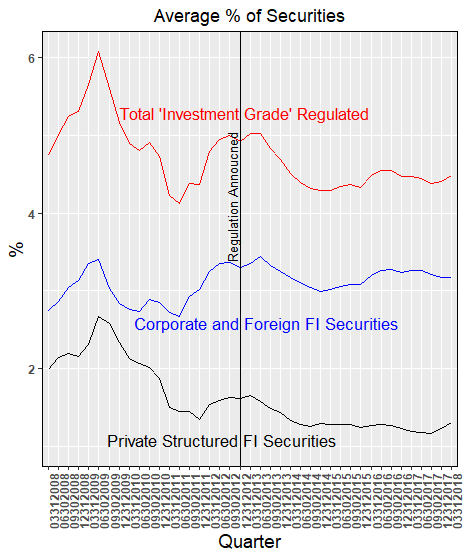
\includegraphics[width = .59999\linewidth]{Rplot}
\end{figure}

Figure \ref{Figure 2} below highlights the sample time series cross sectional total ratios for variables outlined above.  For example, in 2008, of all securities outstanding on bank "Call Report" balance sheets, about 30 percent consisted of corporate bonds, foreign debt instruments, and private structured fixed income securities.  Fast forward to quarter one of 2018 and this number is now fifteen percent, almost exclusively derived from a decrease in the private structured fixed income segment.  Figure \ref{Figure 2} also shows total outstanding securities as a percentage of total assets has increased from 15 percent in 2008 to 20 percent today. Thus, U.S. treasuries, municipals, and agency backed securities make up a larger share of bank balance sheets in 2018 than in 2008.  Figure \ref{Figure 2} in combination with Figure \ref{Figure 1} makes clear the dominance of large banks in the securities market.  The time series of cross sectional averages of variables in Figure \ref{Figure 1} is substantially lower than total values in Figure \ref{Figure 2}. 
\begin{figure}[h!]
\centering
\caption{Time Series of Cross Sectional Totals of Key Variables}
\label{Figure 2}
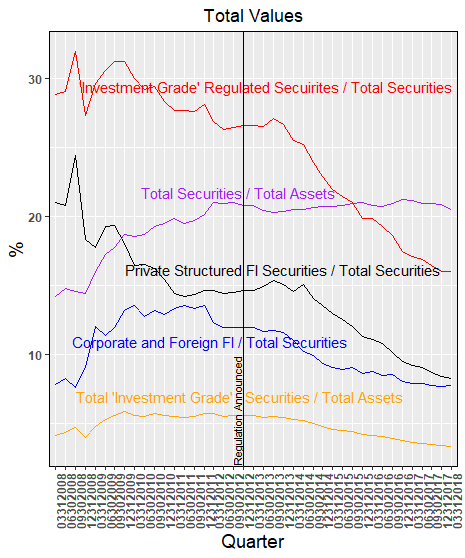
\includegraphics[width = .69\linewidth]{Rplot01}
\end{figure}

\section{Research Design}
The passage of the Dodd–Frank Wall Street Reform and Consumer Protection Act along with the OCC's issuance of revised "investment grade" standards were not exogenous events.  I make no asset pricing claims for newly regulated securities nor do I analyze absolute welfare questions.  Instead, I attempt to identify disproportionate regulatory impact by examining differential security investment between large and small banks.  I measure this impact using the percentage of a bank's security portfolio in securities subject to updated OCC regulations rather than as a percentage of bank total assets.  Using the percentage of a bank's security portfolio in regulated securities controls for confounding issues such as differing lending opportunities.  For example, with small banks' loan portfolios more concentrated in local proximity business loans than large banking institutions, varying geographical economic conditions means differing investment opportunity sets for relationship-based community banks and national transactional focused lenders. Thus, even if a community bank experiences a positive local economic shock unrelated to the new regulation, divestment from securities into newly attractive lending opportunities does not distort my measure of regulatory impact.  A common solution to the issue of geographical heterogeneity is implementing location fixed effects in model specification.  However, fixed effects estimation within a censored panel data Tobit framework I use for regulatory analysis produces inconsistent coefficient estimates \citep{Neyman1948,Lancaster2000}. 

In the scenario above when the small bank has enhanced local lending opportunities, divestment from one security over another to fund new loans is still a reflection of bank security portfolio selection.  A key identifying assumption for differential regulatory impact analysis is that small and large banks' access to purchase securities has not evolved over time.  Identification relies on covariate interactions with a time dummy for periods following regulatory announcement.  Consequently, sample period changes in security purchase ability between small and large banks unrelated to the regulation would confound differential security investment decisions.  Accurate hypothesis testing does not rely on certain banks having more or less favorable access to security investments, but identification does require that any differences in bank access have not changed over time.

The welfare implications of OCC "investment grade" standards concern small banks with locally concentrated asset portfolios.  Small banks may reduce local market risk by investing in assets uncorrelated with local lending conditions such as securities newly affected by the regulation.  However, a bank shifting its securities portfolio away from corporate bonds, foreign debt instruments, and structured securities does not guarantee a bank has reduced its susceptibility to local economic shocks.  For instance, a corporate bond dependent on the general credit quality of the issuer could add to bank local market risk if the issuer's business activities are regionally concentrated within the scope of a bank's lending operations.  On the other hand, securities subject to revised regulations may provide exposure to international markets \footnote{FFIEC "Call Reports" do not provide security level data, so I do not further categorize "investment grade" regulated securities into U.S. and international divisions.} or corporations serving unique markets, both of which are unavailable in securities not required to comply with OCC standards. 

To resolve the uncertain welfare implications of security portfolio selection, I assume bank managers both before and after the regulation allocate their security portfolios to optimize bank location on the risk-return frontier.  I recognize the weakness of the risk-return optimality assumption given managerially incentives to depart from profit maximization or reduction of risk.  Still, the analysis is valid if distorted bank manager objectives did not change over the sample period.  In addition, banks face the friction of information and monitoring duplication for large security issuances such as corporate bonds or private structured securities, but prior to new regulations credit rating agencies helped mitigate this friction.  Consequently, differential divestment between community and large banks from "investment grade" regulated securities, which face information and monitoring duplication frictions due to both size and complexity, indicates a prior disproportionate value of NRSRO's to small banks.  Differential divestments disproportionately reduce the breadth of securities held by small banks compared to large depository institutions.  Last, higher differential divestment among small banks signals further departure from security portfolio optimality than big banks.  This optimality departure is especially important for small firms who rely on community banks for credit access.  

To formally test differential investment in newly regulated securities, I use a correlated random effects two-sided Tobit model with censoring at 0 and 100 percent.  A latent variable interpretation of the panel Tobit model adapted from \citep{Wooldridge2010} is as follows.
\begin{align*}
&y_{it}^{*} = \bm{x}_{it}^{'}\bm{\beta} + \text{c}_{i} + u_{it}, & &y_{it} = 0 \text{ if } y^{*} \leq 0 \nonumber \\
&y_{it} = y^{*} \text{ if } 0 < y^{*} < 100, & &y_{it} = 100 \text{ if } y^{*} \geq 100 \nonumber \\
&c_{i} = \psi + \overline{\bm{x}_{[i]}}^{'}\bm{\zeta} + a_{i} & 
\\
&\\
&\textbf{Assumptions:} \\
&c_{i} \ | \ \bm{x}_{i} \ \sim \ \text{Normal(} \psi + \overline{\bm{x}_{[i]}}^{'}\bm{\zeta}, \ \sigma_{a}^{2} \text{)}, & &u_{it} \ | \ \bm{x}_{i}, a_{i} \ \sim \ \text{Normal(} 0, \sigma_{u}^{2} \text{)} \\
&a_{i} \ | \ \bm{x}_{i} \ \sim \ \text{Normal(} 0, \sigma^{2}_{a} \text{)}, & &(u_{i1},..,u_{iT}) \ | \ (\bm{x}_{i},a_{i}) \ \textrm{Independent}  
\end{align*} 
\begin{align*}
& y_{it}^{*} = \text{Percentage of a Bank's Security Portfolio in Regulated Securities}  \\ 
\\
& \bm{x}_{it}^{'} = (log(Total Assets_{it}), \ \ log(Total Assets_{it})^{2},  \\
& controls_{it}, \ \ After06302012Dummy_{it}, \\
& log(TotalAssets_{it})(After06302012Dummy_{it}), \\
& log(TotalAssets_{it})^{2}(After06302012Dummy_{it}), \\
&(controls_{it})(After06302012Dummy_{it}), \\ 
\\
&\overline{\bm{x}_{[i]}} ^{'} =  \ \overline{(log(Total Assets_{i})}, \ \ \overline{(log(Total Assets_{i})^{2})}, \ \ \overline{(Controls_{i})} \  \
\end{align*} \\
The index "$i$" stands for each bank in the sample, and the index "$t$" represents each quarter from quarter one of 2008 until quarter one of 2018.  Coefficient estimates on $log(TotalAssets_{it})$*$(After06302012Dummy_{it})$ and $log(TotalAssets_{it})^{2}$*$(After06302012Dummy_{it})$ identify the marginal impact of increasing bank size on investment in regulated securities of interest during the regulatory period.  Bank-quarter observations following quarter two of 2012 are chosen as the specification regulatory period because banks were expected to start implementing updated regulatory requirements immediately upon the OCC announcement in June of 2012 \citep{Curry2012}.  The heavily skewed nature of bank total assets calls for a natural log transformation, and a quadratic term is included to account for the decreasing increasing efficiency returns to scale in bank size \citep{Jacewitz2012}. Within the specification, $c_{i}$ accounts for individual bank unobserved heterogeneity, and \bm{$\overline{x_{[i]}}}$ contains all non-constant covariates to account for correlation of individual bank heterogeneity with explanatory variables \citep{Wooldridge2010}.  To clarify the meaning of $\overline{\bm{x}_{[i]}}$, $\overline{ln(Total \ Assets_{i})}$ is simply the average of $ln(Total \ Assets_{it})$ for each bank within the sample time period, so $\overline{ln(Total \ Assets_{i})}$ takes the same value for ($y_{i1}$, $y_{i2}$, ...... $y_{i,T}$).  Next, $a_{i}$ is the conditionally normally distributed error term in bank "$i$" individual heterogeneity $c_{i}$ with variance $\sigma_{a}^{2}$ and zero expected value.  Last, $u_{it}$ is the conditionally normally distributed error term for each bank-quarter observation with variance $\sigma_{u}^{2}$ and zero expected value.      

I use multiple control variables to control for potential endogeneity. A bank's percentage of securities investments in corporate bonds, foreign government debt, and private structured securities is a function of its risk tolerance, so the specification error term includes risk appetite.  %Riskier banks have lower levels of capital (Merton 1977).% 
If risk tolerance has any correlation with bank size, the coefficients on $log(TotalAssets)$ and $log(TotalAssets)^2$ along with coefficients on the time dummy interaction with $log(TotalAssets)$ and $log(TotalAssets)^2$  would be biased. As an imperfect proxy for risk tolerance, $controls_{it}$ includes banks' $Tier1 \ Leverage$ $Ratios$, and $Total$ $Capital$ $Ratios$.  For both metrics, higher percentages signal increased bank resilience to negative balance sheet shocks.  Lower percentages indicate increased bank risk tolerance. 

Omitting bank regulatory capital ratios would create an additional source of endogeneity.  For all else equal, a bank with a regulatory binding low capital ratio will be less able to hold a security portfolio consisting of corporate bonds, foreign debt instruments, or private structured securities.  These securities largely carry higher risk weights under the Basel framework than alternative security investments such as U.S. treasuries or municipal general obligation bonds \citep{RiskWeightsTool}.  Consequently, binding bank capital ratios are a component of the error term in the specified Tobit model.  Any correlation between capital ratios and total bank assets would bias the coefficient estimates of interest. 

Additional $controls_{it}$ variables include $Return$ $on$ $Equity$, $Return$ $on$ $Assets$, and $Efficiency \ Ratio \ Percentages$.  The three metrics gauge bank profitability and efficiency in relation to bank equity, assets, and generated income, respectively.  Ratios such as $Return \ on \ Equity$ are ubiquitous in the banking industry as key performance indicators for bank managers.  Falling short of profitability benchmarks might induce bank executives to strive for additional income by shifting securities investments into higher yielding assets such as emerging market debt or private structured fixed income securities.  As a result, the error term of the specified two-sided Tobit model includes bank managers' desire to achieve concrete profitability and efficiency ratios.  Any correlation between bank size and $ROE$, $ROA$, or $Efficiency$ $Ratios$ would bias coefficient estimates for $ln(TotalAssets)$ and $ln(TotalAssets)^{2}$ and associated interaction terms.  

$ROE$, $ROA$, or $Efficiency$ $Ratios$ also control for bank risk tolerance present in the specification error term. Efficient banks repeatedly earning large returns possess high charter value.  Banks earning excess returns have strong incentives to lower failure probability to continue extracting economic rents.  If a bank does not need to hold securities subject to new OCC regulations for diversification benefits, then consistent high income relative to expenses, assets, or equity might drive bank managers to divest from higher default probability securities such as corporate bonds into U.S. treasuries. Thus, excluding profitability and efficiency metrics would bias coefficient estimates if these metrics are correlated with bank size. 

%Following paragraph is pretty awful, include or not?% 

Another source of possible endogeneity is bank loan geographic diversification.  Banks with geographically concentrated loan portfolios could have differing optimal security portfolio allocations than banks who originate loans nationwide, and loan portfolio diversification is correlated with bank size.  Still, given the previously described heterogeneous nature of assets falling into the category of newly regulated securities, it is not clear having a less diversified loan portfolio implies the optimal bank security portfolio includes more or less "investment grade" regulated securities.  As a result, I have omitted measures of loan diversification such as the annual FDIC "Summary of Deposits" filed by all insured banks, an imperfect measure of individual loan location.  

Given the latent variable model assumptions above, the log likelihood function for $y_{it} \ | \ \bm{x}_{it}^{'}$ is as follows \citep{Bruno2004}. 

\begin{align*}
& L_{i} = \Bigg\{   \int_{-\infty}^{+\infty}  \prod_{t=1}^{T_{i}} \bigg[ \Phi \bigg( \frac{0 -\bm{x}_{it}^{'}\bm{\beta} - \psi - \overline{\bm{x}_{[i]}}^{'}\bm{\zeta}}{\sigma_{u}}\bigg)\bigg]^{I_{it}^{0}}* \\
&\bigg[ \Phi \bigg( \frac{\bm{x}_{it}^{'}\bm{\beta} +\psi + \overline{\bm{x}_{[i]}}^{'}\bm{\zeta} - 100} {\sigma_{u}} \bigg) \bigg] ^{I_{it}^{100}}* \\
& \bigg[ \frac{1}{\sigma_{u}}  \phi \bigg( \frac{y_{it} - \bm{x_{it}}^{'}\bm{\beta} - \psi - \overline{\bm{x}_{[i]}}^{'}\bm{\zeta}}{\sigma_{u}} \bigg) \bigg] ^{(1 - I_{it}^{0} - I_{it}^{100})} \Bigg\} * \phi \bigg( \frac{a_{i}}{\sigma_{a}} \bigg) da_{i} 
\end{align*}
\begin{align*}
&\textrm{log} L = \sum_{i=1}^{N} \textrm{log} L_{i} \\
&\\
& I_{it}^{0}=% 
   \begin{cases}
     1 \ \textrm{if} \ y_{it} \leq0 \\
     0 \ \textrm{if} \ y_{it} > 0 
   \end{cases},
   \qquad 
   I_{it}^{100} =
   \begin{cases}
   	1 \ \textrm{if} \ y_{it} \geq100 \\ 
    0 \ \textrm{if} \ y_{it} < 100
   \end{cases} \\
   &
\end{align*}

The symbols $\phi()$ and  $\Phi()$  are respectively the probability density function (pdf) and 
the cumulative distribution function (cdf) of the standard normal distribution.  I calculate integrals in the log-likelihood function using the Gauss-Hermite quadrature technique, and I maximize the log-likelihood function using the Berndt-Hall-Hall-Hausman (BHHH) algorithm with the "censReg" package in "R" statistical software to estimate to estimate $\bm{\hat{\beta}}$,
$\hat{\psi}$, $\bm{\hat{\zeta}}$, $\hat{\sigma_{a}^{2}}$, and $\hat{\sigma_{u}^{2}}$ \citep{Henningsen2017}.

If the conditional independence of the error term $u_{it}$ is relaxed to allow for serial dependence and individual heterogeneity, $c_{i}$, is ignored, the model can be estimated using a pooled Tobit model.  The latent variable interpretation and log-likelihood function for the pooled model is as follows. 

\begin{align*}
&y_{i}^{*} = \bm{x}_{i}^{'}\bm{\beta} + \epsilon_{i} & &y_{i} = 0 \text{ if } y^{*} \leq 0 \\
&y_{i} = y^{*} \text{ if } 0 < y^{*} < 100, & &y_{i} = 100 \text{ if } y^{*} \geq 100 \\ 
& \epsilon_{i} \ | \ \bm{x}_{i}  \ \sim \ \text{Normal(} 0, \sigma_{\epsilon}^{2} \text{)}, \\
\end{align*}
\begin{align*}
& \textrm{log}L = \sum_{i=1}^{i=N} \bigg[ I_{i}^{0}  \textrm{log}  \Phi \bigg( \frac{0-\bm{x}_{i}^{'}\bm{\beta}}{\sigma_{\epsilon}}\bigg) + I_{i}^{100}  \textrm{log}  \Phi \bigg( \frac{\bm{x}_{i}^{'}\bm{\beta} - 100}{\sigma_{\epsilon}} \bigg) \ + \\
&\bigg( 1 - I_{i}^{0} - I_{i}^{100} \bigg) \bigg( \textrm{log} \phi \bigg( \frac{y_{i} - \bm{x}_{i}^{'}\bm{\beta}}{\sigma_{\epsilon}} \bigg) - \textrm{log} \sigma_{\epsilon} \bigg) \bigg] \\
&
\end{align*}
Each observation "$i$" is a bank-quarter observation with no time distinction, and $\epsilon_{i}$ is the conditionally normally distributed error term for each observation with variance $\sigma_{\epsilon}^{2}$ and zero expected value.  I maximize this log-likelihood function using Newton-Raphson numerical approximation to estimate $\hat{\bm{\beta}}$ and $\hat{\sigma_{\epsilon}}$.

\section{Results}
The first column of Table \ref{Table 2} on page \pageref{Table 2} contains the coefficient estimates from the pooled Tobit model that assumes no unobserved bank individual heterogeneity.  The model in the second column specification allows individual heterogeneity within the panel data structure.  Under the null hypothesis that $\sigma_{c}$ = 0, an asymptotic likelihood ratio test rejects the null of no variance in bank unobserved heterogeneity at a zero percent level of significance.  The specification of column two in Table \ref{Table 2} assumes the panel structure log-likelihood function outlined in the previous section with parameter estimates $\bm{\hat{\beta}}$, $\hat{\psi}$, $\bm{\hat{\zeta}}$, $\hat{\sigma_{a}^{2}}$, and $\hat{\sigma_{u}^{2}}$ , but under the null $\bm{\zeta} = 0$.  Econometrics literature labels this model as a "random effects" panel Tobit specification, and assumes unobserved bank individual heterogeneity is uncorrelated with explanatory covariates.  Column three of Table \ref{Table 2} models correlation between covariates and unobserved bank heterogeneity by placing no restrictions on $\bm{\zeta}$.  The asymptotic likelihood ratio test of the null $\bm{\zeta} = 0$ leads me to reject the "random effects" model in favor of "correlated random effects" model at a zero percent level of significance.  As a result, the model in column three is used to evaluate differential regulatory impact.  

\begin{table}[!htbp] \centering 
  \caption{Coefficient estimates using the two-sided censored Tobit models described in the research design.  Standard errors in parentheses are computed from the observed information matrix from MLE Theory.  Results for the constant coefficient $\hat{\psi}$ are withheld.} 
  \label{Table 2} 
\tiny
\begin{tabular}{@{\extracolsep{5pt}}lD{.}{.}{-3} D{.}{.}{-3} D{.}{.}{-3} } 
\\[-1.8ex]\hline 
\hline \\[-1.8ex] 
 & \multicolumn{3}{c}{\textit{Dependent variable:}} \\ 
\cline{2-4} 
\\[-1.8ex] & \multicolumn{3}{c}{\% Securities Subject to New Regulations}  \\ 
\\[-1.8ex] & \multicolumn{1}{c}{(1)(Pooled Tobit)} & \multicolumn{1}{c}{(2)(Panel Tobit)} & \multicolumn{1}{c}{(3)(Panel Tobit)}\\ 
\hline \\[-1.8ex] 
 $\overline{Log(Total \ Assets_{i})}$ &  &  & -0.776^{**} \\ 
  &  &  & (0.392) \\ 
  & & & \\
 $\overline{log(Total \ Assets_{i})^{2}}$ &  &  & 0.100^{***} \\ 
  &  &  & (0.015) \\
  & & & \\
 $\overline{(Tier1 \ Leverage \ Capital \ Ratio \ \%)_{i}}$ &  &  & 0.025^{***} \\ 
  &  &  & (0.009) \\
  & & & \\
 $\overline{(Total \ RiskBased \ Capital \ Ratio \ \%)_{i}}$ &  &  & -0.002 \\ 
  &  &  & (0.003) \\
  & & & \\
 $\overline{ROE \%{i}}$ &  &  & -0.001 \\ 
  &  &  & (0.001) \\
  & & & \\
 $\overline{ROA \%{i}}$ &  &  & 0.083^{**} \\ 
  &  &  & (0.035) \\
  & & & \\
 $\overline{Efficiency Ratio Percentage_{i}}$ &  &  & 0.003^{***} \\ 
  &  &  & (0.001) \\
  & & & \\
 $Log(Total \ Assets)$ & 3.346^{***} & 12.991^{***} & 16.031^{***} \\ 
  & (0.518) & (0.197) & (0.311) \\
  & & & \\
 $Log(Total \ Assets)^{2}$ & 0.086^{***} & -0.315^{***} & -0.484^{***} \\ 
  & (0.020) & (0.007) & (0.012) \\
  & & & \\
 $Tier1 \ Leverage \ Capital \ Ratio\%$ & 0.101^{***} & -0.019^{***} & -0.032^{***} \\ 
  & (0.009) & (0.003) & (0.004) \\
  & & & \\
 $Total \ RiskBased \ Capital \ Ratio\%$ & -0.00001 & 0.001^{***} & -0.002^{***} \\ 
  & (0.0004) & (0.0002) & (0.0004) \\
  & & & \\
 $ROE\%$ & -0.00005 & 0.00003 & 0.00004 \\ 
  & (0.0001) & (0.0002) & (0.0003) \\
  & & & \\
 $ROA\%$ & -0.189^{***} & 0.295^{***} & 0.306^{***} \\ 
  & (0.051) & (0.014) & (0.015) \\
  & & & \\
 $Efficiency \ Ratio \%$ & -0.0002 & 0.0001 & 0.0001 \\ 
  & (0.0001) & (0.0001) & (0.0001) \\
  & & & \\
 $After06302012Dummy$ & -3.796 & -9.294^{***} & -10.510^{***} \\ 
  & (4.780) & (0.852) & (0.854) \\ 
  & & & \\
 $Log(Total \ Assets)*After06302012Dummy$ & 0.550 & 1.151^{***} & 1.272^{***} \\ 
  & (0.716) & (0.125) & (0.126) \\  
  & & & \\
$Log(Total \ Assets)^{2}*After06302012Dummy$ & -0.048^{*} & -0.055^{***} & -0.054^{***} \\ 
  & (0.027) & (0.005) & (0.005) \\ 
  & & & \\
$(Tier1 \ Leverage \ Capital \ Ratio\%) * (After06302012Dummy)$ & 0.367^{***} & 0.128^{***} & 0.126^{***} \\ 
  & (0.018) & (0.003) & (0.003) \\ 
  & & & \\
 $(Total \ RiskBased \ Capital \ Ratio\%) * (After06302012Dummy)$ & -0.117^{***} & -0.014^{***} & -0.012^{***} \\ 
  & (0.005) & (0.0004) & (0.0005) \\ 
  & & & \\
 $(ROE\%) * (After06302012Dummy)$ & -0.002 & 0.002^{**} & 0.002^{**} \\ 
  & (0.001) & (0.001) & (0.001) \\  
  & & & \\
 $(ROA\%) * (After06302012Dummy)$ & 0.565^{***} & -0.356^{***} & -0.387^{***} \\ 
  & (0.058) & (0.019) & (0.023) \\ 
  & & & \\
 $(Efficiency \ Ratio\%) * (After06302012Dummy)$ & -0.0004 & -0.0004 & -0.002^{**} \\ 
  & (0.0004) & (0.001) & (0.001) \\ 
  & & & \\
 $log(\sigma_{\epsilon})$ & 3.140^{***} &  &  \\ 
  & (0.002) &  &  \\ 
 $log(\sigma_{a})$ &  & 3.100^{***} & 3.116^{***} \\ 
  &  & (0.002) & (0.002) \\ 
 $log(\sigma_{u})$ &  & 2.448^{***} & 2.449^{***} \\ 
  &  & (0.0003) & (0.0003) \\ 
\hline \\[-1.8ex] 
Observations & \multicolumn{1}{c}{270,617} & \multicolumn{1}{c}{270,617} & \multicolumn{1}{c}{270,617} \\ 
Log Likelihood & \multicolumn{1}{c}{-558,093.500} & \multicolumn{1}{c}{-445,186.500} & \multicolumn{1}{c}{-445,120.300} \\ 
\hline 
\hline \\[-1.8ex] 
\textit{Note:}  & \multicolumn{3}{l}{$^{*}$p$<$0.1; $^{**}$p$<$0.05; $^{***}$p$<$0.01} \\ 
 & \multicolumn{3}{l}{} \\ 
\end{tabular} 
\end{table}

The coefficients on the two variables of interest, $log(TotalAssets)$ * \\ $(After$$06302012$$Dummy)$ and $log(TotalAssets)^{2}$ * $(After06302012Dummy)$, are both statically significant.  Still, large panel data sets are notorious for achieving statical significance even if the economic implications are meaningless.  A positive sign on $log(TotalAssets)$*$(After06302012Dummy)$ and negative sign on $log(TotalAssets)^{2}$*$(After06302012Dummy)$ would appear to imply smaller banks differentially divesting "investment grade" regulated securities during the post regulatory period but at a decreasing rate.  The direction of the coefficients aligns with my initial hypothesis.  However, to truly find the differing regulatory impact between small and large bank security portfolios, I need the \textit{difference} between two partial effects of $E[y|\bm{x}]$.  First, I need the partial effect of changes in bank total assets on $E[y|\bm{x}]$ evaluated when $(After06302012Dummy)=1$.  Next, I must also compute the partial effect for an increase in total assets when $(After06302012Dummy)=0$.  The difference between these two partial effects identifies the regulatory impact on differential security investment levels between small and large banks. The analytical expression for partial effects at the average for an increase in total assets for the two sided "correlated random effects" Tobit model in column three of Table \ref{Table 2} is as follows.

\begin{align*}
& \bigg( \hat{\beta}_{log(TotalAssets)} \ + \ 2\hat{\beta}_{log(TotalAssets)^{2}}(log(TotalAssets)) \ + \\ 
& \hat{\beta}_{log(TotalAssets)*(After06302012Dummy)} \ + \\ 
& 2\hat{\beta}_{log(TotalAssets)^{2}*(After06302012Dummy)}(log(TotalAssets))\bigg) * \\ 
& \bigg( \Phi \Big(\frac{100 -  \hat{\psi} - \overline{\bm{x}}^{'}\hat{\bm{\beta}} - \overline{\overline{\bm{x}_{i}}}^{'}\hat{\bm{\zeta}}}{\hat{\sigma}_{u}} \Big) -  \Phi \Big(\frac{0 -  \hat{\psi} - \overline{\bm{x}}^{'}\hat{\bm{\beta}} - \overline{\overline{\bm{x}_{i}}}^{'}\hat{\bm{\zeta}}}{\hat{\sigma}_{u}} \Big) \bigg) * \\
& log(\frac{AssetsNew}{AssetsOld}) \\ 
&
\end{align*}

When $(After06302012Dummy)=1$, the vector $\overline{\bm{x}}^{'}$ contains the average of each control variable in the entire sample.  Each average is in the $\overline{\bm{x}}^{'}$ vector twice due to the existence of interaction terms.  In addition, $log(TotalAssets)$ and $log(TotalAssets)^{2}$ are each in the vector $\overline{\bm{x}}^{'}$ twice, but I manually choose their values.  Next, $\overline{\overline{\bm{x}_{i}}}^{'}$ is a vector of averages of each individual bank average variable.  $\hat{\sigma}_{u}$ is the point estimate of the standard deviation of the non-individual random component in every $y_{it}$ observation. The bottom row of column three in Table 2 contains the estimate for $log(\sigma_{u})$.   For computing partial effects when $(After06302012Dummy)=0$, elements from $\overline{\bm{x}}^{'}$ only appear once due to the elimination of the interaction terms.  Also, the terms
\begin{align*}
&\hat{\beta}_{log(TotalAssets)(After06302012Dummy)}, \\ &2\hat{\beta}_{log(TotalAssets)^{2}*(After06302012Dummy)}(log(TotalAssets))
\end{align*}
are zero. At any selected value of $TotalAssets$, differential regulatory impact is identified by the partial effect at the average when $(After06302012Dummy)$ $=1$ minus the partial effect at the average when $(After06302012Dummy)=0$.  %\cite{Jacewitz2012} a majority of community banking economies of scale improvement is achieved by the time the bank possess between 100 and 300 million of total assets.% 

For welfare analysis, I am concerned with community banks, often defined as banks with less than \$1 billion in total assets.  The 1st percentile of banks as measured by total assets for all bank-quarter observations in the sample had about \$12 million in total assets.  I compute the difference in partial effects at the average for $TotalAsset$ levels from \$12 million to \$1 billion in \$20 million increments assuming a doubling of banks $TotalAssets$ for each partial effect.  The doubling assumption makes the $log(\frac{AssetsNew}{AssetsOld})$ term in the partial effects formula equal $ln(2)$.  In the 50 regulatory impact computations, the largest result predicts a 0.02 percentage \textit{decrease} in the conditional expected percentage of a bank's total securities in newly regulated securities for a doubling of banks assets.  The minimum regulatory impact predicts a 0.17 percent \textit{decrease}.  Both estimates are economically insignificant and the opposite direction of my hypothesis. 

Partial effects at the average may produce erroneous results if covariate control variable averages for the entire sample do not reflect community bank characteristics.  In response, I also estimate regulatory impact using the difference of average partial effects for two sub-samples of data.  I place all quarters after quarter two of 2012 into a "post regulatory" sample, and the remaining observations into a "prior to regulation" sample.  Next, within each sample, I exclude bank-quarter observations with more than \$1 billion in total assets. The following is the analytical expression for average partial effects for a two-sided pooled Tobit model adapted from \cite{Wooldridge2010,Wooldridge2013} for the specification in column three of Table 2.

\begin{align*}
& \frac{1}{n} \sum_{k=1}^{k=n} \bigg( \hat{\beta}_{log(TotalAssets)} \ + \ 2\hat{\beta}_{log(TotalAssets)^{2}}(log(TotalAssets_{k})) \ +\\ 
& \hat{\beta}_{log(TotalAssets)*(After06302012Dummy)} \ + \\ 
& 2\hat{\beta}_{log(TotalAssets)^{2}*(After06302012Dummy)}(log(TotalAssets_{k}))\bigg) * \\ 
& \bigg( \Phi \Big(\frac{100 -  \hat{\psi} - \bm{x}_{k}^{'}\hat{\bm{\beta}} - \overline{\bm{x}_{i}}^{'}\hat{\bm{\zeta}}}{\sqrt[]{(\hat{\sigma}_{u}^{2} \ + \ \hat{\sigma}_{a}^{2})}} \Big) -  \Phi \Big(\frac{0 -  \hat{\psi} - \bm{x}_{k}^{'}\hat{\bm{\beta}} - \overline{\bm{x}_{i}}^{'}\hat{\bm{\zeta}}}{\sqrt[]{(\hat{\sigma}_{u}^{2} \ + \ \hat{\sigma}_{a}^{2})}} \Big) \bigg) * \\
& log(\frac{AssetsNew}{AssetsOld}) \\ 
&
\end{align*}

The sum of $k=1$ to $k=n$ indicates each bank-quarter observation in the subsample.  For example, in the "post regulatory" period when \\ $(After$$06302012$$Dummy)=1$, every observation with less than \$1 billion in total assets falling after quarter 2 of 2012 is averaged.  The expression $ \hat{\psi} - \bm{x}_{k}^{'}\hat{\bm{\beta}} - \overline{\bm{x}_{i}}^{'}\hat{\bm{\zeta}}$ is the predicted value for each bank-quarter observation $k$ in the subsample.  To clarify, $ \overline{\bm{x}_{i}}^{'}$ varies on bank identification index $i$ for each observation $k$.  $\hat{\sigma}_{a}^{2}$ is the estimated variance of the individual error component, and this estimate is shown in the second to last row in column three of Table 2.  The terms 
\begin{align*}
&\hat{\beta}_{log(TotalAssets)*(After06302012Dummy)}, \\ 
&2\hat{\beta}_{log(TotalAssets)^{2}*(After06302012Dummy)}(log(TotalAssets))
\end{align*}
are zero in the average partial effects computation for the "prior to regulation" subsample when the $(After$$06302012$$Dummy)=0$. 

The average partial effect during the "post regulatory" period for banks with less than \$1 billion in total assets for a doubling of total assets is a 0.83 percent expected increase in the percentage of a bank's security portfolio invested in newly regulated securities. During the "prior to regulation" period, the average partial effect computation produces an expected increase of 0.93 percent.  In total, the average partial effect of doubling bank size on the expected percentage of bank securities facing "investment grade" standards attributable to the regulation is a \textit{decrease} of 0.09 percent, an economically insignificant number. 

Figure \ref{Figure 3} below is a histogram of all Table \ref{Table 2} dependent variable bank-quarter observations.  
\begin{figure}[htpb!]
\centering
\caption{}
\label{Figure 3}
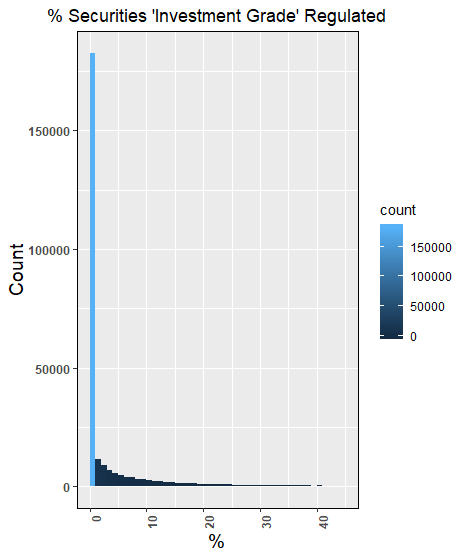
\includegraphics[width = .5\linewidth]{Rplot02}
\end{figure}
The horizontal axis is separated into 1\% width buckets, and the vertical axis is the count for the number of observations in each bucket.  Of the 270,617 observations in the sample period, 166,093 hold no corporate bonds, foreign debt instruments, or private structured securities.  In both the average partial effects and partial effects at the average calculations, the second half of the expression is a correction term representing the probability of observing an uncensored response \citep{Wooldridge2013}.  In the case of average partial effects, the average of $k=1$ to $k=n$ correction terms is .28 for the post regulatory period and .30 for the pre-regulatory period.  As a result, coefficient point estimates are non-materially reduced for economic significance evaluation. 


As a robustness check, I repeat the analysis setting $y_{it}^{*}$ equal to the percentage of a bank's security portfolio in private structured securities.  I also estimate a correlated random effects Tobit model with $y_{it}^{*}$ equal to the percentage of a bank's security portfolio in corporate and foreign fixed income instruments.  Private structured securities dependent on underlying cash flows from a variety of assets are often more challenging to analyze than a bond whose repayment likelihood relies on the general credit quality of the issuer.  Thus, the OCC's new "investment grade" standards are likely more difficult to implement for structured products.  Higher differential divestment in private structured products than corporate and foreign fixed income securities between small and large banks is plausible.  The results from setting $y_{it}^{*}$ equal to the percentage of a bank's security portfolio in private structured securities can be seen in Table \ref{Table 3} on page \pageref{Table 3}. 



%%%%%%%Table for Private Structured Securities: 
\begin{table}[!htbp] \centering 
  \caption{Coefficient estimates using the two-sided censored Tobit models described in the research design.  Standard errors in parentheses are computed from the observed information matrix from MLE Theory.  Results for the constant coefficient $\hat{\psi}$ are withheld.} 
  \label{Table 3} 
\tiny 
\begin{tabular}{@{\extracolsep{5pt}}lD{.}{.}{-3} D{.}{.}{-3} D{.}{.}{-3} } 
\\[-1.8ex]\hline 
\hline \\[-1.8ex] 
 & \multicolumn{3}{c}{\textit{Dependent variable:}} \\ 
\cline{2-4} 
\\[-1.8ex] & \multicolumn{3}{c}{\% Securities Private Structured FI} \\ 
\\[-1.8ex] & \multicolumn{1}{c}{(1)(Pooled Tobit)} & \multicolumn{1}{c}{(2)(Panel Tobit)} & \multicolumn{1}{c}{(3)(Panel Tobit)}\\ 
\hline \\[-1.8ex] 
 $\overline{Log(Total \ Assets_{i})}$ &  &  & -4.661^{***} \\ 
  &  &  & (0.471) \\ 
  & & & \\ 
 $\overline{log(Total \ Assets_{i})^{2}}$ &  &  & 0.275^{***} \\ 
  &  &  & (0.017) \\ 
  & & & \\ 
 $\overline{(Tier1 \ Leverage \ Capital \ Ratio \ \%)_{i}}$ &  &  & 0.124^{***} \\ 
  &  &  & (0.016) \\ 
  & & & \\ 
 $\overline{(Total \ RiskBased \ Capital \ Ratio \ \%)_{i}}$ &  &  & 0.002 \\ 
  &  &  & (0.005) \\ 
  & & & \\ 
 $\overline{ROE \%{i}}$ &  &  & 0.002 \\ 
  &  &  & (0.003) \\ 
  & & & \\ 
 $\overline{ROA \%{i}}$ &  &  & 0.205^{***} \\ 
  &  &  & (0.042) \\ 
  & & & \\ 
 $\overline{Efficiency Ratio Percentage_{i}}$ &  &  & 0.004^{***} \\ 
  &  &  & (0.001) \\ 
  & & & \\ 
 $Log(Total \ Assets)$ & 10.430^{***} & 12.102^{***} & 19.767^{***} \\ 
  & (0.566) & (0.231) & (0.365) \\ 
  & & & \\ 
 $Log(Total \ Assets)^{2}$ & -0.154^{***} & -0.299^{***} & -0.665^{***} \\ 
  & (0.021) & (0.008) & (0.014) \\ 
  & & & \\ 
 $Tier1 \ Leverage \ Capital \ Ratio\%$ & -0.171^{***} & -0.175^{***} & -0.257^{***} \\ 
  & (0.018) & (0.004) & (0.005) \\ 
  & & & \\ 
 $Total \ RiskBased \ Capital \ Ratio\%$ & 0.001^{***} & 0.001^{***} & -0.0003 \\ 
  & (0.0004) & (0.0003) & (0.001) \\ 
  & & & \\ 
 $ROE\%$ & -0.0001 & 0.0001 & 0.0003 \\ 
  & (0.0001) & (0.0001) & (0.0005) \\ 
  & & & \\ 
 $ROA\%$ & -0.101 & -0.018 & -0.057^{***} \\ 
  & (0.062) & (0.016) & (0.017) \\ 
  & & & \\ 
 $Efficiency \ Ratio \%$ & 0.0005 & 0.0002 & 0.0001 \\ 
  & (0.0005) & (0.0003) & (0.0003) \\ 
  & & & \\ 
 $After06302012Dummy$ & 1.580 & -28.654^{***} & -31.705^{***} \\ 
  & (5.351) & (1.139) & (1.182) \\ 
  & & & \\ 
 $Log(Total \ Assets)*After06302012Dummy$ & -0.978 & 2.921^{***} & 3.195^{***} \\ 
  & (0.783) & (0.163) & (0.170) \\ 
  & & & \\ 
 $Log(Total \ Assets)^{2}*After06302012Dummy$ & 0.023 & -0.097^{***} & -0.097^{***} \\ 
  & (0.029) & (0.006) & (0.006) \\ 
  & & & \\ 
 $(Tier1 \ Leverage \ Capital \ Ratio\%) * (After06302012Dummy)$ & 0.239^{***} & 0.227^{***} & 0.225^{***} \\ 
  & (0.026) & (0.005) & (0.006) \\ 
  & & & \\ 
 $(Total \ RiskBased \ Capital \ Ratio\%) * (After06302012Dummy)$ & -0.022^{***} & -0.002^{***} & 0.002^{***} \\ 
  & (0.005) & (0.0004) & (0.0005) \\ 
  & & & \\ 
 $(ROE\%) * (After06302012Dummy)$ & -0.0003 & 0.006^{***} & 0.006^{***} \\ 
  & (0.002) & (0.001) & (0.001) \\ 
  & & & \\ 
 $(ROA\%) * (After06302012Dummy)$ & 0.710^{***} & -0.060^{***} & -0.074^{**} \\ 
  & (0.069) & (0.021) & (0.032) \\ 
  & & & \\ 
 $(Efficiency \ Ratio\%) * (After06302012Dummy)$ & -0.0001 & -0.0001 & -0.00003 \\ 
  & (0.001) & (0.001) & (0.001) \\ 
  & & & \\ 
 $log(\sigma_{\epsilon})$ & 3.035^{***} &  &  \\ 
  & (0.004) &  &  \\ 
 $log(\sigma_{a})$ &  & 3.059^{***} & 3.065^{***} \\ 
  &  & (0.004) & (0.004) \\ 
 $log(\sigma_{u})$ &  & 2.375^{***} & 2.377^{***} \\ 
  &  & (0.0003) & (0.0004) \\ 
\hline \\[-1.8ex] 
Observations & \multicolumn{1}{c}{270,617} & \multicolumn{1}{c}{270,617} & \multicolumn{1}{c}{270,617} \\ 
Log Likelihood & \multicolumn{1}{c}{-288,224.400} & \multicolumn{1}{c}{-218,960.700} & \multicolumn{1}{c}{-218,831.500} \\ 
\hline 
\hline \\[-1.8ex] 
\textit{Note:}  & \multicolumn{3}{l}{$^{*}$p$<$0.1; $^{**}$p$<$0.05; $^{***}$p$<$0.01} \\ 
 & \multicolumn{3}{l}{} \\ 
\end{tabular} 
\end{table} 

The three model specifications in Table \ref{Table 3} are identical to Table \ref{Table 2}.  I reject the first two column specifications in favor of the third column correlated random effects model at 0\% levels of significance for both likelihood ratio tests previously described.  The coefficients on the variables of interest, $log(TotalAssets)$*$(After06302012Dummy)$ and \\ $log(TotalAssets)^{2}$*$(After06302012Dummy)$ are both statically significant, and I repeat the partial effects at the average and average partial effects calculations outline above.  In 50 partial effects at the average regulatory impact computations for a doubling of bank total assets, the maximum result predicts \textit{no} change in a bank's conditional expected percentage of securities held in private structured fixed income products.  The minimum partial effects at the average computation predicts a .01 percentage expected \textit{decrease}.  Average partial effects analysis produces similar results.  The difference between the post and pre-regulatory average partial effects for community banks when bank assets double predicts a \textit{decrease} of .042 percent in a bank's expected percentage of total securities in private structured investments attributable to the regulation.  Economically insignificant results come from the large percentage of bank-quarter observations censored at zero.  220,179 of the 270,617 bank-quarter observations in the sample period hold no private structured securities. In the case of average partial effects, the average correction term is 0.088 for the post regulatory period and 0.119 for the period prior to regulatory announcement. 

The specifications in Table \ref{Table 4} on page \pageref{Table 4} set $y_{it}^{*}$ to the percentage of a bank's security portfolio in corporate and foreign fixed income instruments.  The correlated random effects model in column three is used for regulatory evaluation after rejecting column one and two specifications at 0\% levels of significance.  The interaction variables of interest on $TotalAssets$ are statistically significant, but the previously used partial effects methods predict economically insignificant regulatory impact.  Among the 50 partial effects at the average regulatory impact computations, the maximum result predicts \textit{no} change in a bank's conditional expected percentage of securities held in corporate and foreign fixed income instruments.  The minimum partial effects at the average computation predicts a .048 percentage expected \textit{decrease}.  The difference between the post and pre-regulatory average partial effects for community banks when bank total assets double predicts a \textit{decrease} of 0.036 percent in a bank's expected percentage of total securities in corporate and foreign fixed income securities.  For a third time, economically meaningless partial effects are a function of bank-quarter observations censored at zero.  188,920 of 270,617 bank-quarter observations in the sample period hold no corporate or foreign fixed income investments producing small correction terms.  In conclusion, there appears to be no discernible difference in differentially regulatory impact for the two subcategories of securities subject to revised regulations. 


%%%%%%%Table for Corporate/Foreign Fixed Income 
\begin{table}[!htbp] \centering 
  \caption{Coefficient estimates using the two-sided censored Tobit models described in the research design.  Standard errors in parentheses are computed from the observed information matrix from MLE Theory.  Results for the constant coefficient $\hat{\psi}$ are withheld.} 
  \label{Table 4} 
\tiny 
\begin{tabular}{@{\extracolsep{5pt}}lD{.}{.}{-3} D{.}{.}{-3} D{.}{.}{-3} } 
\\[-1.8ex]\hline 
\hline \\[-1.8ex] 
 & \multicolumn{3}{c}{\textit{Dependent variable:}} \\ 
\cline{2-4} 
\\[-1.8ex] & \multicolumn{3}{c}{\% Securities Corporate and Foreign FI} \\ 
\\[-1.8ex] & \multicolumn{1}{c}{(1)(Pooled Tobit)} & \multicolumn{1}{c}{(2)(Panel Tobit)} & \multicolumn{1}{c}{(3)(Panel Tobit)}\\ 
\hline \\[-1.8ex] 
 $\overline{Log(Total \ Assets_{i})}$ &  &  & -0.535 \\ 
  &  &  & (0.422) \\ 
  & & & \\ 
 $\overline{Log(Total \ Assets_{i})^{2}}$ &  &  & 0.048^{***} \\ 
  &  &  & (0.016) \\ 
  & & & \\ 
 $\overline{(Tier1 \ Leverage \ Capital \ Ratio \ \%)_{i}}$ &  &  & 0.014^{*} \\ 
  &  &  & (0.007) \\ 
  & & & \\ 
 $\overline{(Total \ RiskBased \ Capital \ Ratio \ \%)_{i}}$ &  &  & 0.001 \\ 
  &  &  & (0.002) \\ 
  & & & \\ 
 $\overline{ROE \%{i}}$ &  &  & -0.001 \\ 
  &  &  & (0.001) \\ 
  & & & \\ 
 $\overline{ROA \%{i}}$ &  &  & -0.042 \\ 
  &  &  & (0.028) \\ 
  & & & \\ 
 $\overline{Efficiency Ratio Percentage_{i}}$ &  &  & 0.001 \\ 
  &  &  & (0.001) \\ 
  & & & \\ 
 $Log(Total \ Assets)$ & 2.748^{***} & 2.876^{***} & 3.958^{***} \\ 
  & (0.501) & (0.197) & (0.363) \\ 
  & & & \\ 
 $Log(Total \ Assets)^{2}$ & 0.039^{**} & 0.016^{**} & -0.047^{***} \\ 
  & (0.019) & (0.007) & (0.014) \\ 
  & & & \\ 
 $Tier1 \ Leverage \ Capital \ Ratio\%$ & 0.203^{***} & 0.052^{***} & 0.049^{***} \\ 
  & (0.011) & (0.001) & (0.001) \\ 
  & & & \\ 
 $Total \ RiskBased \ Capital \ Ratio\%$ & -0.049^{***} & -0.087^{***} & -0.088^{***} \\ 
  & (0.005) & (0.001) & (0.001) \\ 
  & & & \\ 
 $ROE\%$ & -0.00002 & -0.00002 & 0.0001 \\ 
  & (0.0001) & (0.0004) & (0.0002) \\ 
  & & & \\ 
 $ROA\%$ & 0.015 & 0.434^{***} & 0.449^{***} \\ 
  & (0.052) & (0.012) & (0.013) \\ 
  & & & \\ 
 $Efficiency \ Ratio \%$ & -0.0002^{**} & 0.0001 & 0.0001 \\ 
  & (0.0001) & (0.0001) & (0.0001) \\ 
  & & & \\ 
 $After06302012Dummy$ & -13.697^{***} & -0.990 & -1.302 \\ 
  & (4.644) & (0.970) & (0.980) \\ 
  & & & \\ 
 $Log(Total \ Assets)*After06302012Dummy$ & 1.957^{***} & 0.278^{*} & 0.314^{**} \\ 
  & (0.693) & (0.147) & (0.149) \\ 
  & & & \\ 
 $Log(Total \ Assets)^{2}*After06302012Dummy$ & -0.086^{***} & -0.024^{***} & -0.023^{***} \\ 
  & (0.026) & (0.006) & (0.006) \\ 
  & & & \\ 
 $(Tier1 \ Leverage \ Capital \ Ratio\%) * (After06302012Dummy)$ & 0.592^{***} & 0.212^{***} & 0.209^{***} \\ 
  & (0.023) & (0.005) & (0.005) \\ 
  & & & \\ 
 $(Total \ RiskBased \ Capital \ Ratio\%) * (After06302012Dummy)$ & -0.191^{***} & -0.070^{***} & -0.069^{***} \\ 
  & (0.010) & (0.002) & (0.002) \\ 
  & & & \\ 
 $(ROE\%) * (After06302012Dummy)$ & -0.002 & 0.001 & 0.0004 \\ 
  & (0.001) & (0.002) & (0.002) \\ 
  & & & \\ 
 $(ROA\%) * (After06302012Dummy)$ & -0.639^{***} & -0.468^{***} & -0.465^{***} \\ 
  & (0.078) & (0.019) & (0.020) \\ 
  & & & \\ 
 $(Efficiency \ Ratio\%) * (After06302012Dummy)$ & -0.002 & -0.001 & -0.002^{**} \\ 
  & (0.002) & (0.001) & (0.001) \\ 
  & & & \\ 
 $log(\sigma_{\epsilon})$ & 3.068^{***} &  &  \\ 
  & (0.003) &  &  \\ 
 $log(\sigma_{a})$ &  & 3.031^{***} & 3.034^{***} \\ 
  &  & (0.002) & (0.002) \\ 
 $log(\sigma_{u})$ &  & 2.347^{***} & 2.348^{***} \\ 
  &  & (0.0003) & (0.0003) \\ 
\hline \\[-1.8ex] 
Observations & \multicolumn{1}{c}{270,617} & \multicolumn{1}{c}{270,617} & \multicolumn{1}{c}{270,617} \\ 
Log Likelihood & \multicolumn{1}{c}{-448,117.500} & \multicolumn{1}{c}{-346,397.600} & \multicolumn{1}{c}{-346,376.100} \\ 
\hline 
\hline \\[-1.8ex] 
\textit{Note:}  & \multicolumn{3}{l}{$^{*}$p$<$0.1; $^{**}$p$<$0.05; $^{***}$p$<$0.01} \\ 
 & \multicolumn{3}{l}{} \\ 
\end{tabular} 
\end{table} 

Figure \ref{Figure 4} on page \pageref{Figure 4} is a stylistic representation of differential regulatory impact analysis between small and large banks.  For each quarter, I separate banks into ten deciles based on $TotalAssets$.  Figure \ref{Figure 4} plots the difference between the average of the 10th Decile (largest) and 1st Decile (smallest) bank's percentage of securities portfolio subject to the OCC's updated regulation.  A decrease over time indicates large and small banks average security portfolio percentages converging while increases represent large banks on average holding more newly regulated securities than small community banks.  

\begin{figure}[h!]
\centering
\caption{}
\label{Figure 4}
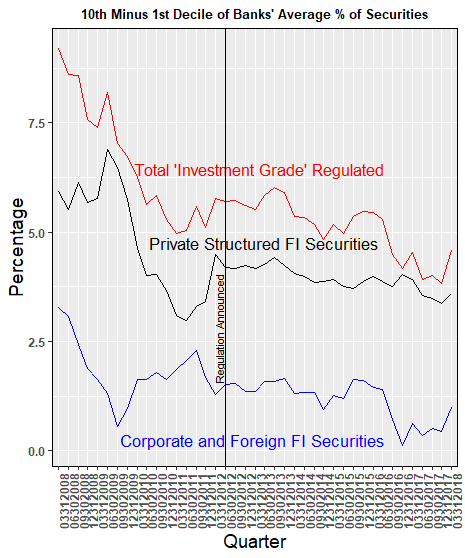
\includegraphics[width = .7\linewidth]{Rplot07}
\end{figure}

The time series reveals larger banks have had a higher percentage of their securities portfolios in "investment grade" regulated securities for the entire sample period.  Following the 2008 financial crisis, the difference between small and large bank's average percentage of securities in newly regulated securities decreased by about 2 to 3 percentage points.  This difference has actually \textit{decreased} further since regulatory announcement, albeit by only about one percentage point.  Immediately prior to the announcement of the regulation in June of 2012, banks in the tenth decile held on average between 5 and 6 percent more of their securities portfolio in securities now subject to additional regulatory scrutiny than banks in the 1st decile.  With the regulation in effect, the difference has dropped to between 4 and 5 percent.  Figure \ref{Figure 4} aligns with both the unexpected direction and economically insignificant results of the two-sided correlated random effects Tobit Model partial effect regulatory impact computations.  The indiscernible difference between the two subcategories of "investment grade" regulated securities produced by the Tobit models in Tables \ref{Table 3} and \ref{Table 4} also fits Figure \ref{Figure 4}.  For further information, see Figures \ref{Figure 5}, \ref{Figure 6} and \ref{Figure 7} in the Appendix.  These figures plot the time series for the average percentage of total bank securities in "investment grade" type securities and its two subcategories for all ten bank size deciles.  


\section{Conclusion}
Empirical evidence suggests the OCC's revised "investment grade" standards issued to comply with Dodd-Frank Act Section 939A have not differentially altered small and large bank security portfolios.  Assuming all bank managers allocate their security portfolios to optimize risk and return trade-offs, the regulation has not disproportionately shifted small banks from security portfolio optimality.  Through the channel of bank security selection, neither large nor small bank borrowers have been more nor less burdened by the regulation.  As anecdotal evidence, I interned at a bank in 2012 preparing to implement OCC standards, and I recently corresponded with the bank Chief Financial Officer.  The CFO stated the regulation has had little impact on security portfolio selection.  The bank's "investment grade" documentation for pre-purchase analysis is a basic checklist.  For securities in the bank's current portfolio, broker provided quarterly performance reports satisfy regulatory requirements.   Finally, I take no position on overall welfare implications of the new rules.  

\section{Appendix} 
\subsection{Variable Creation}
Table \ref{Table 5} on page \pageref{Table 5} outlines the creation of model variables from FFIEC bank "Call Reports."  Banks with domestic offices file a 041 form while banks with both foreign and domestic offices file a 031 form.  "Call Report" item number and definitions have changed over time, and variable creation for the analysis reflects these changes.  As an example, for banks using form 031, $Total \ Risk\textrm{-}Based \ Capital \ Ratio\%$ changed from "Call Report" item RCFD7205 to RCFA7205 at the beginning of 2015.  Within Table \ref{Table 5} for variable $Total \ Risk\textrm{-}Based \ Capital$ $Ratio\%$ under column "Form 031 Items," I sum "Call Report" items RCFA7205 and RCFD7205 because the two items never exist concurrently.  Please see the data dictionary provided by the Federal Reserve \citep{Reserve2018} for detailed "Call Report" item definitions.  
 
\begin{table}[!htbp] \centering 
  \caption{Variable Creation from FFIEC Bank "Call Report" Items} 
  \label{Table 5} 
  \footnotesize
\begin{tabular} {|m{.33\textwidth}|m{.33\textwidth}|m{.33\textwidth}|}
\hline 
\multicolumn{3}{|c|}{\textbf{Variable Creation Table}} \\
\hline 
 \textbf{Variable} & \textbf{Form 041 Items} & \textbf{Form 031 Items}   \\
 \hline
 
 \%  Securities Newly Regulated & (Regulated Securities) / (Total Securities) & (Regulated Securities) / (Total Securities) \\ 
 \hline
 Regulated Securities & Corporate/Foreign FI + Private Structured FI & Corporate/Foreign FI + Private Structured FI \\
 \hline
 Corporate and Foreign FI Securities & RCON1737 + RCON1742 + RCON1741 + RCON1746 & RCFD1737 + RCFD1742 + RCFD1741 + RCFD1746 \\ 
 \hline
 Private Structured FI Securities & RCON1709 + RCON1713 + RCON1733 + RCON1736 + RCONC026 + RCONC027 + RCONG308 + RCONG320 + RCONK146 + RCONK154 + RCONG324 + RCONG328 + RCONG336 + RCONG340 + RCONG344 + RCONG311 + RCONG323 + RCONK149 + RCONG327 + RCONG331 + RCONK157 + RCONG339 + RCONG343 + RCONG347 & RCFDG308 + RCFD1709 + RCFD1733 + RCFD1713 + RCFD1736 + RCFDG320 + RCFDK146 + RCFDG324 + RCFDK154 + RCFDG328 + RCFDC026 + RCFDG336 + RCFDG340 + RCFDG344 + RCFDG311 + RCFDG323 + RCFDK149 + RCFDG327 + RCFDK157 + RCFDG331 + RCFDC027 + RCFDG339 + RCFDG343 + RCFDG347 \\
 \hline
 Total Securities & RCON1754 + RCON1773 & RCFD1754 + RCFD1773 \\ 
 \hline
 \% Securities Corporate and Foreign FI & (Corporate and Foreign FI Securities) / (Total Securities) & (Corporate and Foreign FI Securities) / (Total Securities) \\ 
 \hline
 \% Securities Private Structured FI & (Private Structured FI Securities) / (Total Securities) & (Private Structured FI Securities) / (Total Securities) \\ 
 \hline
 Efficiency Ratio\% & (Non-Interest Expenses) / (Net Interest Income + Non-Interest Income) & (Non-Interest Expenses) / (Net Interest Income + Non-Interest Income) \\ 
 \hline 
 Non-Interest Expenses & RIAD4093 & RIAD4093 \\ 
 \hline
 Net Interest Income & RIAD4074 & RIAD4074 \\ 
 \hline
 Non-Interest Income & RIAD4079 & RIAD4079 \\ 
 \hline 
 ROE\% & (Net Income) / (Total Equity) & (Net Income) / (Total Equity) \\ 
 \hline
 Net Income & RIAD4340 & RIAD4340 \\ 
 \hline
 Total Equity & Total Assets - Total Liabilities & Total Assets - Total Liabilities \\ 
 \hline
 Total Assets & RCON2170 & RCFD2170 \\ 
 \hline
 Total Liabilities & RCON2948 & RCFD2948 \\ 
 \hline
 ROA\% & (Net Income) / (Total Assets) & (Net Income) / (Total Assets) \\ 
 \hline
 Tier1 Leverage Capital Ratio \% & RCON7204 + RCOA7204 & RCFA7204 + RCFD7204 \\ 
 \hline
 Total Risk-Based Capital Ratio\% & RCON 7205 + RCOA7205 & RCFA7205 + RCFD7205 \\ 
 \hline
\end{tabular}
\end{table}
 
\subsection{Additional Figures}

\begin{figure}[h!]
\centering
\caption{}
\label{Figure 5}
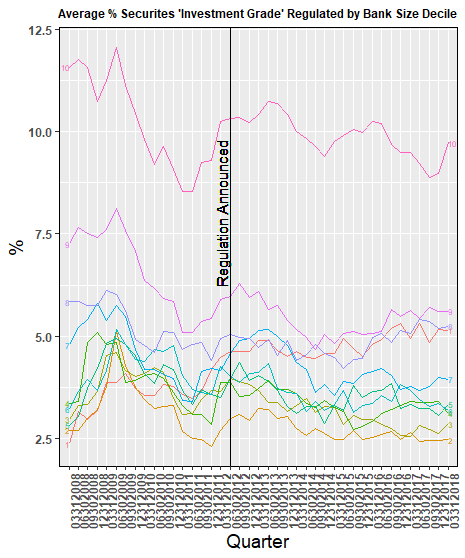
\includegraphics[width = .97\linewidth]{Rplot03}
\end{figure}

\begin{figure}[h!]
\centering
\caption{}
\label{Figure 6}
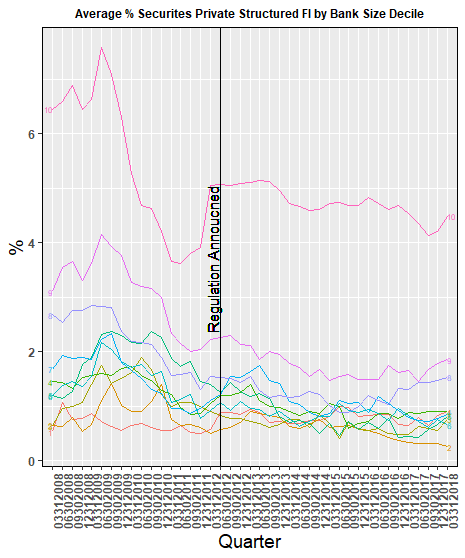
\includegraphics[width = .97\linewidth]{Rplot04}
\end{figure} 

\begin{figure}[h!]
\centering
\caption{}
\label{Figure 7}
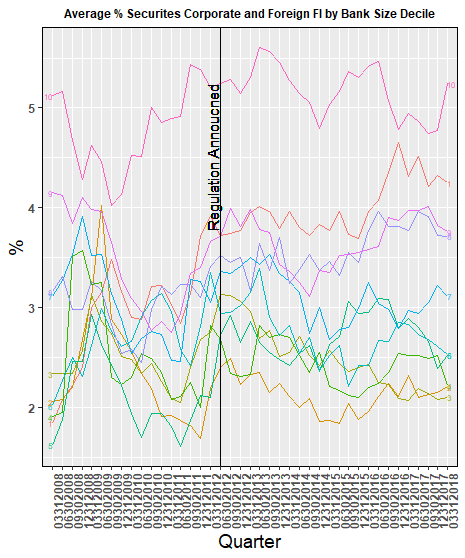
\includegraphics[width = .97\linewidth]{Rplot05}
\end{figure}



%% References
%%
%% Following citation commands can be used in the body text:
%% Usage of \cite is as follows:
%%   \cite{key}          ==>>  [#]
%%   \cite[chap. 2]{key} ==>>  [#, chap. 2]
%%   \citet{key}         ==>>  Author [#]


%% References with bibTeX database:

\clearpage
\pagestyle{plain}
\section*{\refname}
\bibliography{939A_Dodd_Frank}
\bibliographystyle{apalike}




%% Authors are advised to submit their bibtex database files. They are
%% requested to list a bibtex style file in the manuscript if they do
%% not want to use model1-num-names.bst.


%% References without bibTeX database:

% \begin{thebibliography}{00}

%% \bibitem must have the following form:
%%   \bibitem{key}...
%%

% \bibitem{}

% \end{thebibliography}

\end{document}

%%
%% End of file `elsarticle-template-1-num.tex'.